\section{Experiments \& Results}
In this section, the experiments to reach the best tuning parameters and the results will be given for the methods explained in this chapter.
\subsection{Univariate Autoregressive Model}
There are 4 parameters to be optimized in univariate autoregressive modeling method. These parameters are the coefficient degree, AR order, window length and overlap.  \par
Firstly, we will try to answer the question about which AR order and which coefficient order is best. For this purpose, experiments will be done for AR orders from 1 to 15 with three different window length 500, and 50\% overlap. 
\begin{figure}
	\begin{center}
		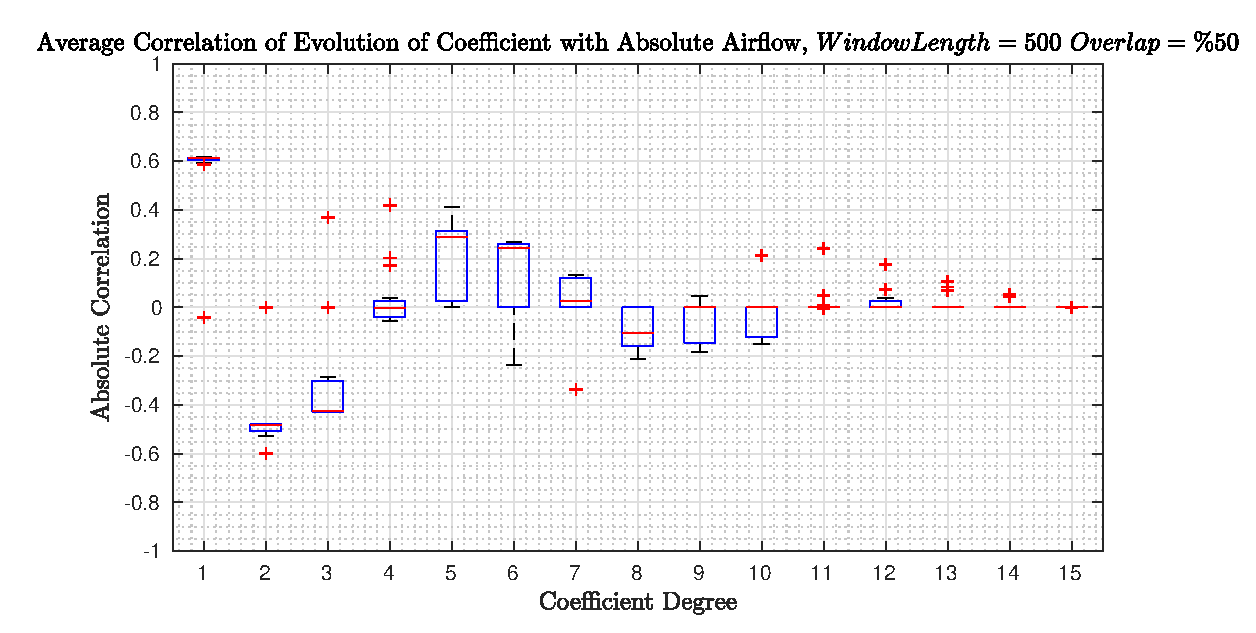
\includegraphics[width=\textwidth]{figures/corr_abs_coeff_for_degree_selection.eps}
		\caption{Boxplot for correlation coefficient of AR coefficient evolution with absolute value of airflow for different coefficient orders}
		\label{fig:absolute_airflow_window_coef}
	\end{center}
\end{figure}
\begin{figure}
	\begin{center}
		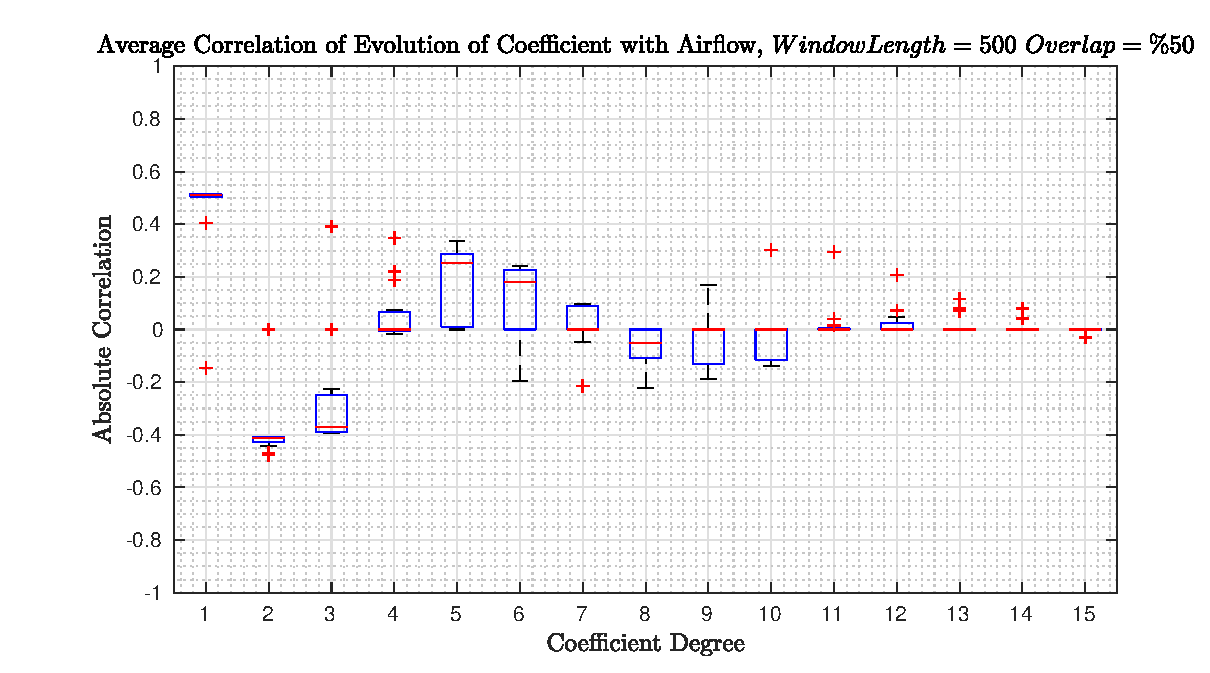
\includegraphics[width=\textwidth]{figures/corr_normal_coeff_for_degree_selection.eps}
		\caption{Boxplot for correlation coefficient of AR coefficient evolution with airflow for different coefficient orders}
		\label{fig:normal_airflow_window_coef}
	\end{center}
\end{figure}
\begin{figure}
	\begin{center}
		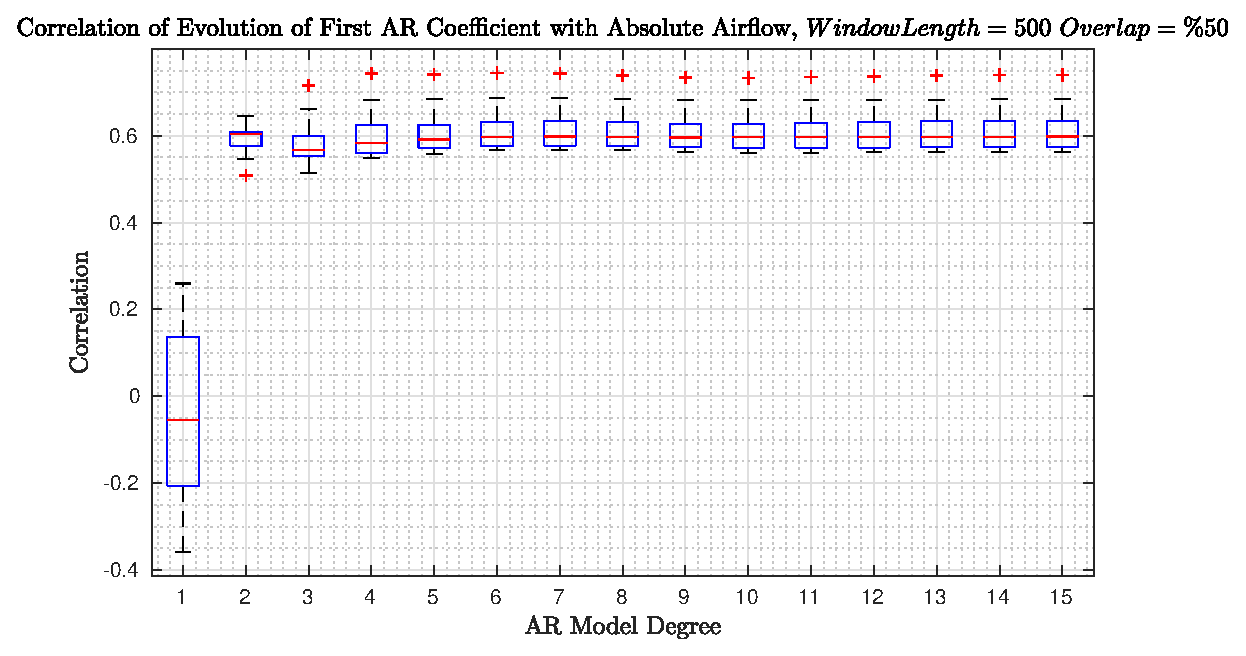
\includegraphics[width=\textwidth]{figures/corr_abs_for_ar_model_degree_selection.eps}
		\caption{Boxplot for correlation coefficient of AR coefficient evolution with airflow for different AR model orders}
		\label{fig:abs_airflow_window_ar_model}
	\end{center}
\end{figure}
\begin{figure}
	\begin{center}
		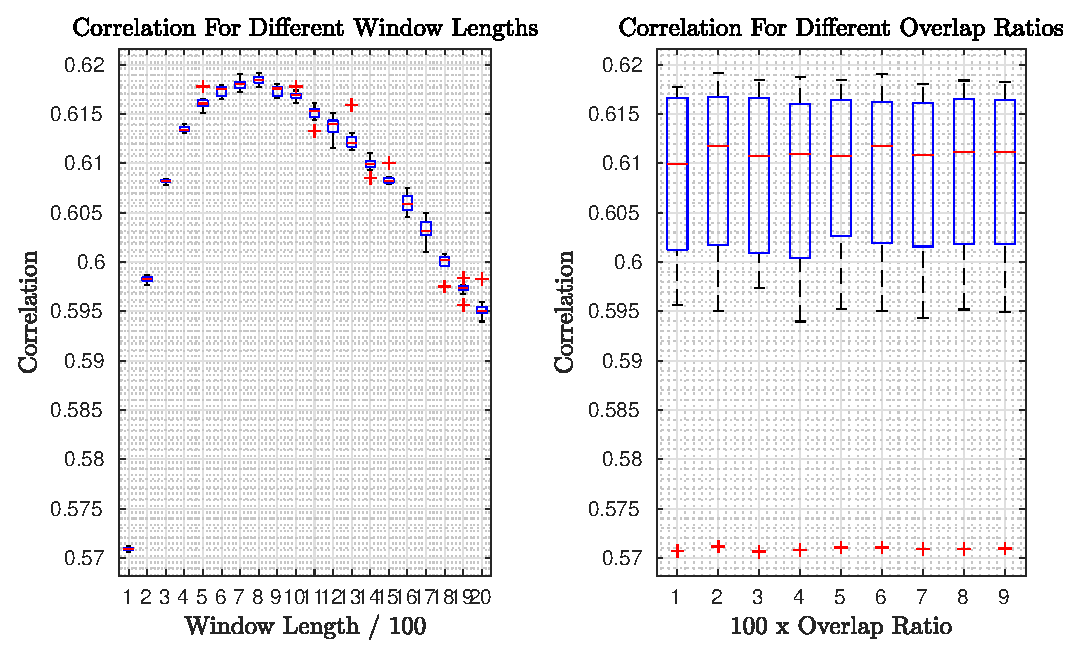
\includegraphics[width=\textwidth]{figures/corr_abs_for_window_length_selection.eps}
		\caption{Boxplot for correlation coefficient of first AR coefficient evolution with absolute airflow for different window lengths and overlap ratios}
		\label{fig:abs_airflow_window_ar_model_window_overlap}
	\end{center}
\end{figure}\par
The inference from figures  is that the correlation is decreasing with increasing coefficient order and the correlation with absolute value of flow is significantly greater. We will continue our analysis with absolute value of airflow for AR estimators. Now we will continue the analysis to find the best model order. For this, we run experiments with window length 500 and an overlap of \%50 with model orders from 1 to 15. The results are shown in figure \ref{fig:abs_airflow_window_ar_model}. As can be seen from figure, there isn't any significant difference after sixth order AR model, so we chose 6 as our model order. After selecting model order, the window length and overlap ratio are left to be decided on. In order to select them we run experiments with window lengths from 100 to 2000 with a seperation of 100 and overlap ratios from 10\% to 90\% with a separation of 10\%. The results for different window lengths and overlap ratios are summarized in figure \ref{fig:abs_airflow_window_ar_model_window_overlap}, according to the results best window length is 800 and difference in overlap ratio doesn't generate any difference in the correlation. We decided to use 90\% overlap to increase the resolution. \par
The resulting decision for univariate autoregressive solution with overlapping windows is 6, 800, 90\% for model order, window length and overlap ratio respectively. 
\subsection{Time Varying Autoregressive Model with Basis Functions}
The parameters for this method are model order, number of basis functions and the frequency difference in adjacent basis functions. \par 
First, we run experiments to determine the best model order and for this purpose run experiments with model orders from 1 to 15 where the number of basis functions are 201 (100 sines, 100 cosines and a constant) and the separation in frequency is 0.04 $Hz$. Experiment results are given in figure \ref{fig:abs_airflow_tvar_model_order}. Most correlation is achieved with the model order of 6 again. \par
After deciding on model order, we need to decide on number of basis functions and frequency separation of basis functions. Before doing this, we run experiments to determine the frequency coverage for best correlation and run experiments with separation of 0.025 $Hz$ and different number of basis frequencies from 50 to 300 with steps of 50. The result is given in figure \ref{fig:abs_airflow_tvar_freq_range}. According to test results 5 $Hz$ is enough to cover for best results.
\begin{figure}
	\begin{center}
		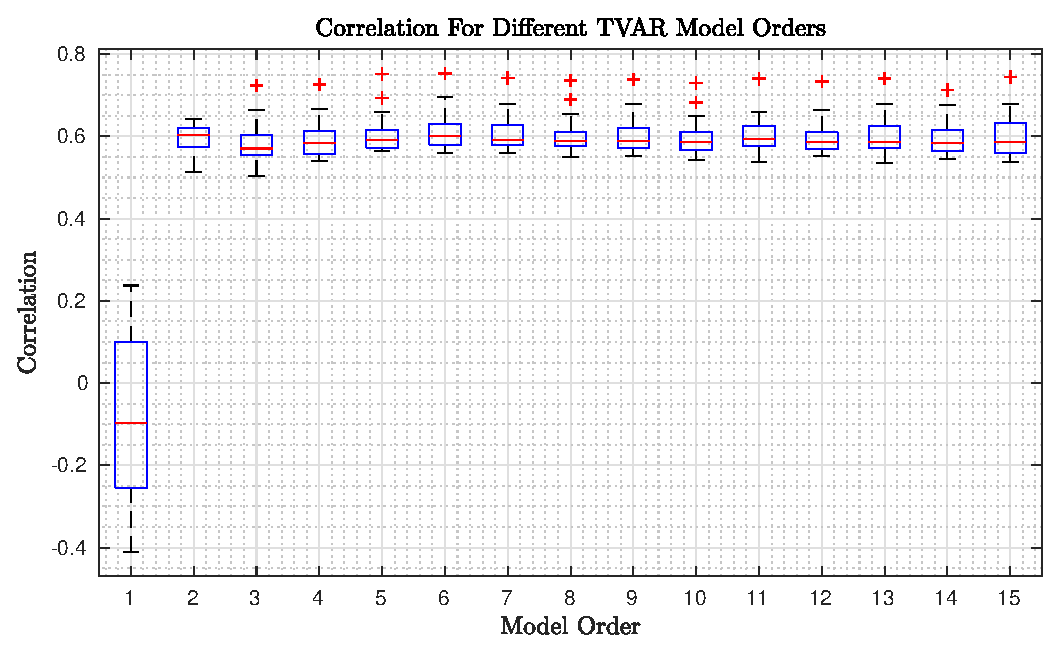
\includegraphics[width=\textwidth]{figures/corr_abs_for_tvar_ar_order_selection.eps}
		\caption{Boxplot for correlation coefficient of first AR coefficient evolution with absolute airflow for different TVAR model orders}
		\label{fig:abs_airflow_tvar_model_order}
	\end{center}
\end{figure}
\begin{figure}
	\begin{center}
		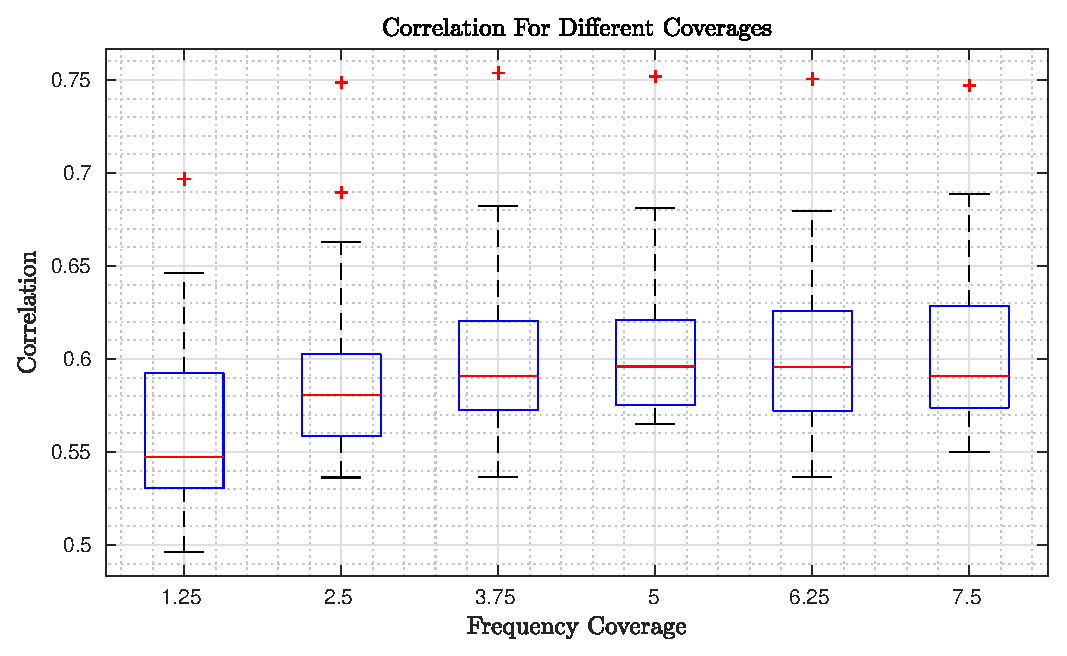
\includegraphics[width=\textwidth]{figures/corr_abs_for_tvar_frange_selection.eps}
		\caption{Boxplot for correlation coefficient of first AR coefficient evolution with absolute airflow for different frequency coverage}
		\label{fig:abs_airflow_tvar_freq_range}
	\end{center}
\end{figure}
Finally we run simulations to decide both the number of basis frequencies and frequency separation and for each tuning we covered the frequency range from 0 to 5 $Hz$. The results are given in figure \ref{fig:abs_airflow_tvar_numbasis_selection}, it shows that it doesn't make significant change to choose number of basis functions as 200 or 400. We chose it to be 250 for minimum standard deviation. \par 
To summarize, 6, 250, 0.02 is chosen for model order, number of basis frequencies and frequency separation respectively.
\begin{figure}
	\begin{center}
		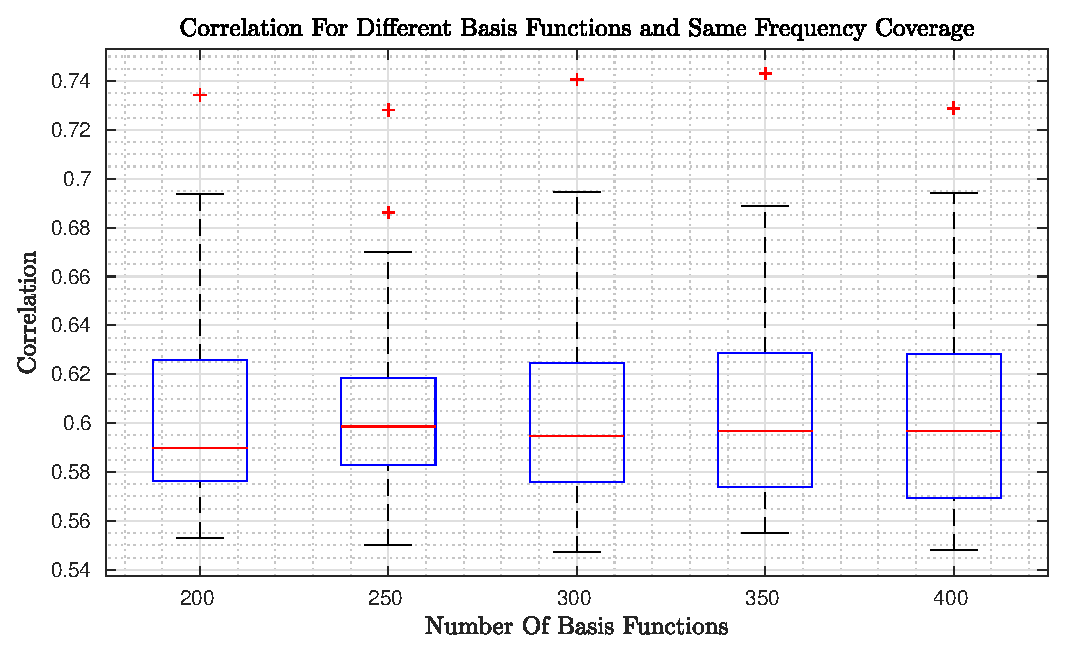
\includegraphics[width=\textwidth]{figures/corr_abs_for_tvar_numbasis_selection.eps}
		\caption{Boxplot for correlation coefficient of first AR coefficient evolution with absolute airflow for number of basis functions}
		\label{fig:abs_airflow_tvar_numbasis_selection}
	\end{center}
\end{figure} \par 

\subsection{Time Varying Autoregressive Model with Kalman Filter}
For this method, we used the noise estimated by windowing based AR modeling as the measurement noise variance, and look for the best noise variance for process noise. We run simulations where the state uncertainity goes from 0.0002 to 0.004 with steps of 0.0002. The results are given in \ref{fig:abs_airflow_kalman_noise_selection}. We chose 0.004 as our process variance.

\begin{figure}
	\begin{center}
		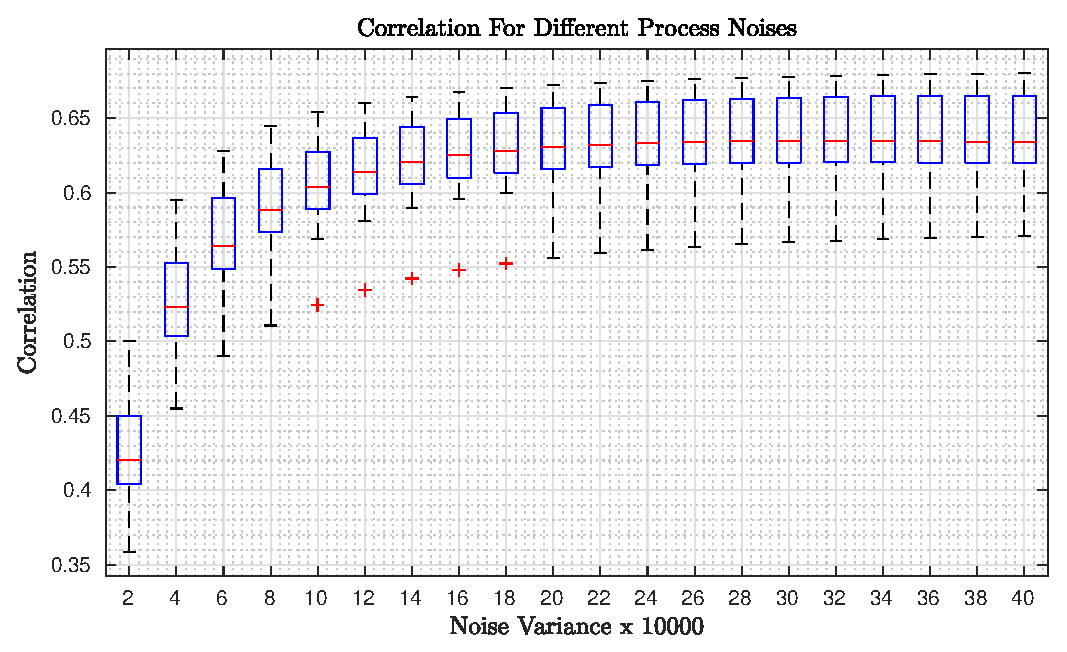
\includegraphics[width=\textwidth]{figures/corr_abs_for_kalman_noise_selection.eps}
		\caption{Boxplot for correlation coefficient of first AR coefficient evolution with absolute airflow for different process noise variances}
		\label{fig:abs_airflow_kalman_noise_selection}
	\end{center}
\end{figure}

\subsection{Short Time Fourier Transform}
\begin{figure}[h!]
	\begin{center}
		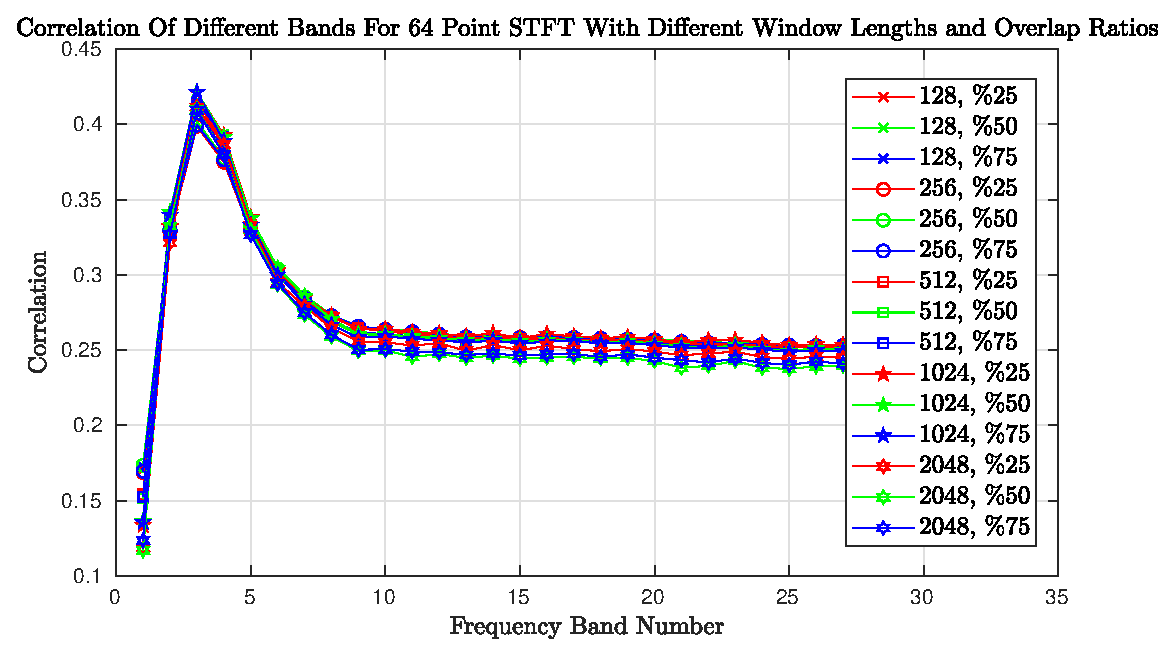
\includegraphics[width=\textwidth]{figures/corr_normal_for_stft_64.eps}
		\caption{Mean of correlations for each band for STFT method with 64 fft bins, window lengths and overlap ratios}
		\label{fig:airflow_stft_64}
	\end{center}
\end{figure}
\begin{figure}[h!]
	\begin{center}
		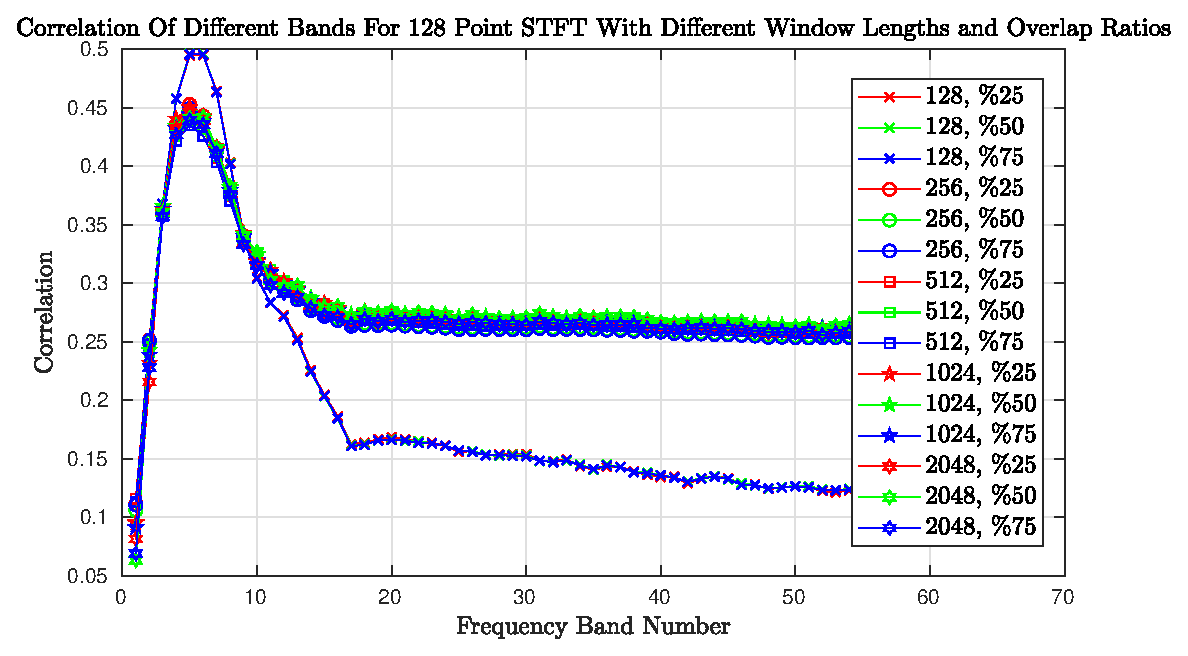
\includegraphics[width=\textwidth]{figures/corr_normal_for_stft_128.eps}
		\caption{Mean of correlations for each band for STFT method with 128 fft bins, window lengths and overlap ratios}
		\label{fig:airflow_stft_128}
	\end{center}
\end{figure}
\begin{figure}[h!]
	\begin{center}
		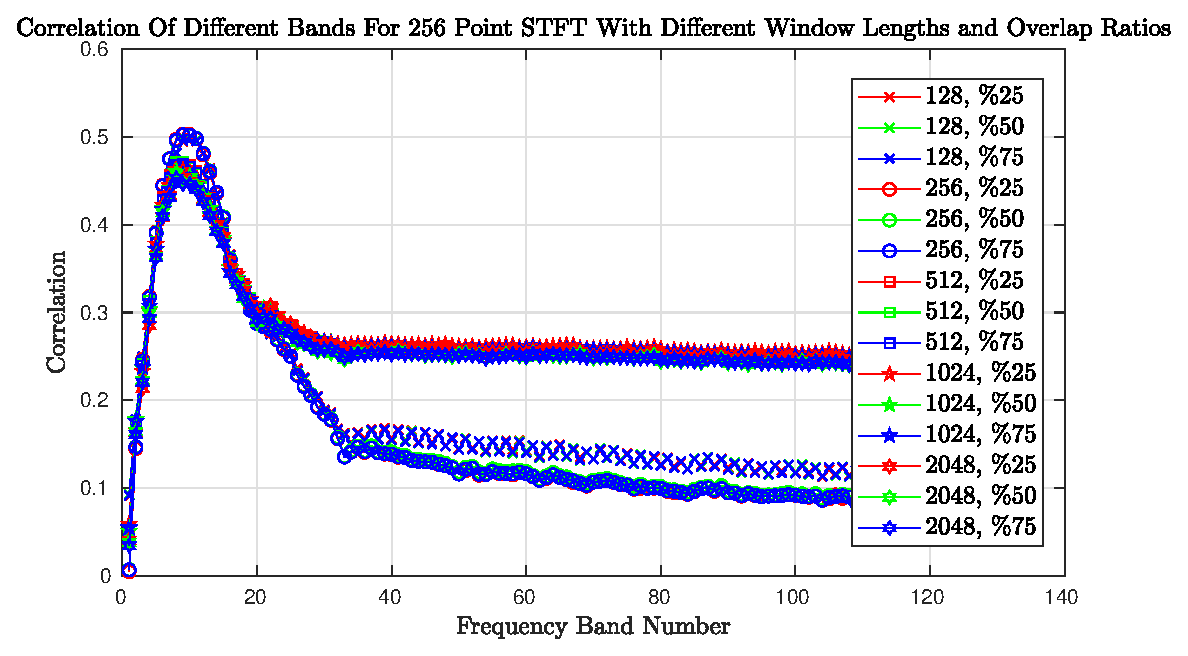
\includegraphics[width=\textwidth]{figures/corr_normal_for_stft_256.eps}
		\caption{Mean of correlations for each band for STFT method with 256 fft bins, window lengths and overlap ratios}
		\label{fig:airflow_stft_256}
	\end{center}
\end{figure}

\subsection{Unifying Estimations}
We run simulations with different number of vectors to be unified, where the vectors are outputs of univariate AR and STFT methods.
\begin{figure}[h!]
	\begin{center}
		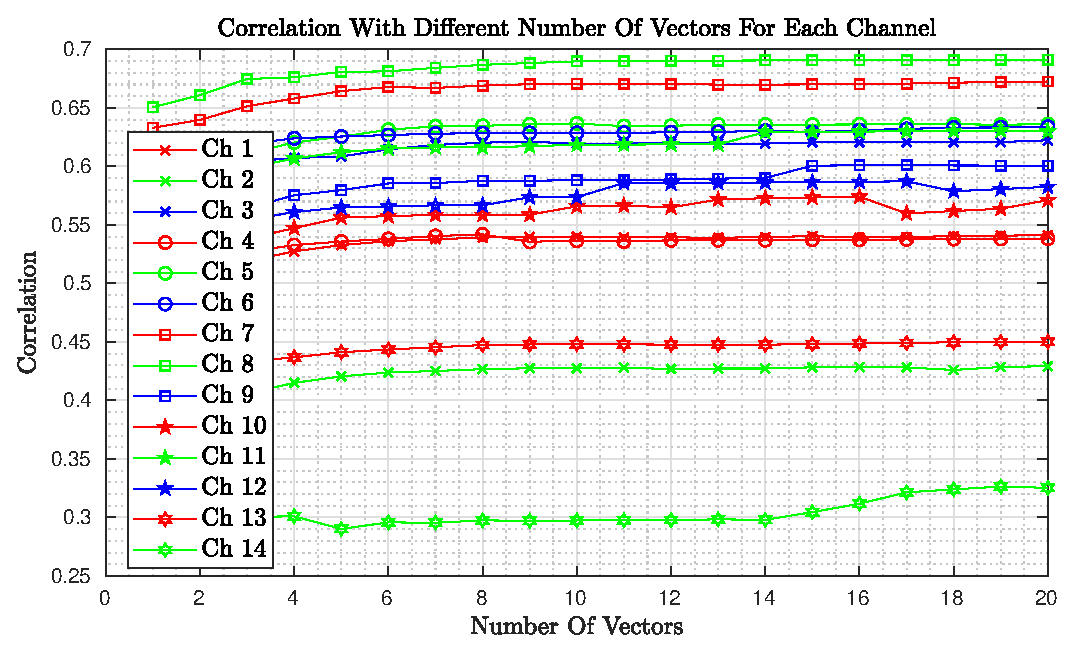
\includegraphics[width=\textwidth]{figures/corr_normal_unify.eps}
		\caption{Mean of correlations for each channel with different number of vectors unified}
		\label{fig:airflow_unify}
	\end{center}
\end{figure}
       

\subsection{Result}
\begin{table}[h!]
	\centering
	\begin{tabular}{|| c c c c ||} 
		\hline
		Channel & Univariate AR & Basis Functions & Kalman \\ [0.5ex] 
		\hline\hline
		1 & 0.6871 & 0.6862 & 0.6290 \\ 
		2 & 0.7440 & 0.7280 & 0.6802 \\
		3 & 0.6800 & 0.6699 & 0.6647 \\
		4 & 0.6310 & 0.6185 & 0.6536\\
		5 & 0.6153 & 0.6047 & 0.6649 \\
		6 & 0.5935 & 0.5963 & 0.6134 \\ 
		7 & 0.6031 & 0.6031 & 0.6328 \\ 
		8 & 0.5980 & 0.5885 & 0.6672 \\ 
		9 & 0.5761 & 0.5828 & 0.6351 \\ 
		10 & 0.5900 & 0.6009 & 0.6328 \\ 
		11 & 0.5681 & 0.5500 & 0.6197 \\ 
		12 & 0.5688 & 0.5719 & 0.6362 \\ 
		13 & 0.5733 & 0.5652 & 0.6127 \\ 
		14 & 0.5952 & 0.5916 & 0.5706 \\ 
		\hline
		\end{tabular}
		\caption{Correlation For Different Methods for All Channels}
		\label{table:1}
\end{table}